\documentclass[14pt]{beamer}


\usepackage{color}
\usepackage{tikz}


\mode<presentation>
{
\usetheme{AlpesLasers}
\setbeamercovered{transparent}
  %\setbeamertemplate{footline}[frame number] 
  %\setbeamertemplate{navigation symbols}{ 
  %\hskip 0.3cm
  %\insertframenumber / \inserttotalframenumber  % <<< frame #
  %\insertpagenumber / \insertpresentationendpage % <<< page #
%} 
}

% font definitions, try \usepackage{ae} instead of the following
% three lines if you don't like this look
\usepackage{listings}
\lstloadlanguages{python}

\usepackage{mathptmx}
\usepackage[scaled=.90]{helvet}
\usepackage{courier}
\usepackage[T1]{fontenc}
\usepackage[english]{babel}
\usepackage[latin1]{inputenc}
\title{Designing an efficient simulation framework}
%\subtitle{A little overview}
\author{St\'ephane Poss}
\date{\today}
% This is only inserted into the PDF information catalog. Can be left
% out.
\subject{PYTHON}

\lstdefinestyle{custompy}{
  belowcaptionskip=1\baselineskip,
  breaklines=true,
  xleftmargin=\parindent,
  language=python,
  showstringspaces=false,
  basicstyle=\footnotesize\ttfamily,
  keywordstyle=\bfseries\color{green!40!black},
  commentstyle=\itshape\color{purple!40!black},
  identifierstyle=\color{blue},
  stringstyle=\color{orange},
}
\lstdefinestyle{customsh}{
  belowcaptionskip=1\baselineskip,
  breaklines=true,
  xleftmargin=\parindent,
  language=bash,
  showstringspaces=false,
  basicstyle=\footnotesize\ttfamily,
  keywordstyle=\bfseries\color{green!40!black},
  commentstyle=\itshape\color{purple!40!black},
  identifierstyle=\color{blue},
  stringstyle=\color{orange},
}
\lstdefinestyle{customcpp}{
  belowcaptionskip=1\baselineskip,
  breaklines=true,
  xleftmargin=\parindent,
  language=C++,
  showstringspaces=false,
  basicstyle=\footnotesize\ttfamily,
  keywordstyle=\bfseries\color{green!40!black},
  commentstyle=\itshape\color{purple!40!black},
  identifierstyle=\color{blue},
  stringstyle=\color{orange},
}

\begin{document}
\begin{frame}[plain]
\titlepage
\end{frame}

\begin{frame}
\tableofcontents
\end{frame}

\section{Motivation}
\begin{frame}
\frametitle{Why this training?}

\end{frame}

\begin{frame}
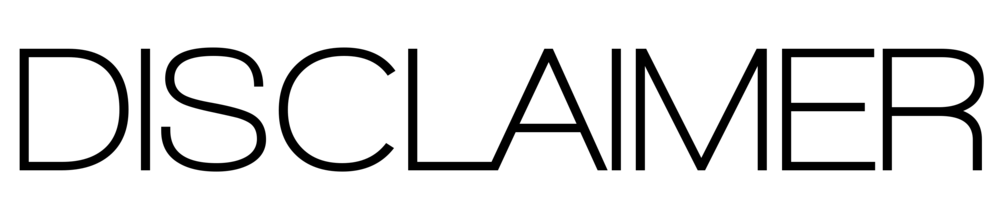
\includegraphics[width=\textwidth]{disclaimer}
\end{frame}

\begin{frame}
\begin{quote}
Maybe it's not worth teaching people this stuff, maybe it's worth for them to discover the do's and don'ts by themselves...
\end{quote}
\end{frame}

\section{Definitions}
\begin{frame}
Definitions
\end{frame}

\begin{frame}
Efficiency
\end{frame}

\begin{frame}
Simulation framework
\end{frame}

\begin{frame}
\frametitle{Why simulations?}
\end{frame}

\section{The usual situation}
\begin{frame}
The situation
\end{frame}
\subsection{1st year PhD}
\begin{frame}
\frametitle{1st year PhD}
\begin{itemize}
\item Create files on the fly, in the same directory
\item Overwrite code, changes drastically every day, DRY principle NOT applied
\item Code monolithic as much as possible: one class (if any at all)
\item Output are named test\_1, test\_2, test\_1\_altered, lum\_check\_260815, plots are all in the same directory
\end{itemize}
\end{frame}

\begin{frame}
\begin{itemize}
\item Application version does not matter, hacked to fit need if possible.
\item Data stored only on personal drive, not backed up
\item Sharing of data via email, but unusable because code base is too messy
\item All analysis are slightly different, can hardly be shared between run points
\end{itemize}
\end{frame}
\subsection{2nd year PhD}
\begin{frame}
\frametitle{2nd year PhD}
\begin{itemize}
\item Use directory structure\\ /data/thesis/simu/260815/param1/param2/file\_param1\_param2.out, input.txt, source code, but variable and rigid (How to add info without moving things around?)
\item Code organized by date: changes imply copy of the code structure
\item Code structured: reused functions appear
\item Application version is checked regularly, new features asked to dev being added on demand (if possible)
\end{itemize}
\end{frame}
\begin{frame}
\begin{itemize}
\item Log book stores results textually-> link between file names and contents
\item Data shared via NFS/FTP/SCP/etc. Code base clearer and can be used by someone trained for a few days. API changes not backward compatible
\item Recipes to process data in place, still done manually
\end{itemize}
\end{frame}

\subsection{3rd year PhD}
\begin{frame}
\frametitle{3rd year PhD}
\begin{itemize}
\item Use DB, graphDB for meta description of data: flexible, extensible, easy to find what you want
\item Files stored on persistent drive (backup, distributed, shared)
\item Synergy with application developer: you ask, they add, you use.
\item Core applications wrapped to store I/O directly in DB
\item Code properly documented, API well defined and stable
\end{itemize}
\end{frame}

\begin{frame}
\begin{itemize}
\item Code is organized in logical elements, core libraries stand out and reused. data structures are decoupled from functions
\item Code versioning used extensively (GIT, SVN)
\item Automatic processing of data: workflows, data driven processing
\item Use code from elsewhere, don't reinvent the wheel
\end{itemize}
\end{frame}

\section{Where we go from there}
\begin{frame}
The tools to proceed
\end{frame}

\subsection{PYTHON}
\begin{frame}
\frametitle{Python}
\end{frame}

\subsection{Coding practices}
\begin{frame}
\frametitle{Code version}
\end{frame}

\begin{frame}
\frametitle{Documentation}
\end{frame}

\subsection{Application control}
\begin{frame}
\frametitle{Manage your applications}
\end{frame}

\subsection{Data storage}
\begin{frame}
\frametitle{Data storage and metadata}
\end{frame}

\begin{frame}
\frametitle{Data base systems}
\end{frame}

\begin{frame}
\frametitle{iRods}
\end{frame}

\end{document}